\subsection {Accelerometer}

The \systemName~includes an ADXL345 3-axis digital accelerometer, which can be used to
measure acceleration on the board in three directions. The Accelerometer chip is controlled by the
Accelerometer SPI Mode core, which provides a memory-mapped interface at address {\sf 0xFF204020}
to {\sf 0xFF204021}, as shown in in Figure~\ref{fig:accel_port}.

\begin{figure}[h!]
   \begin{center}
       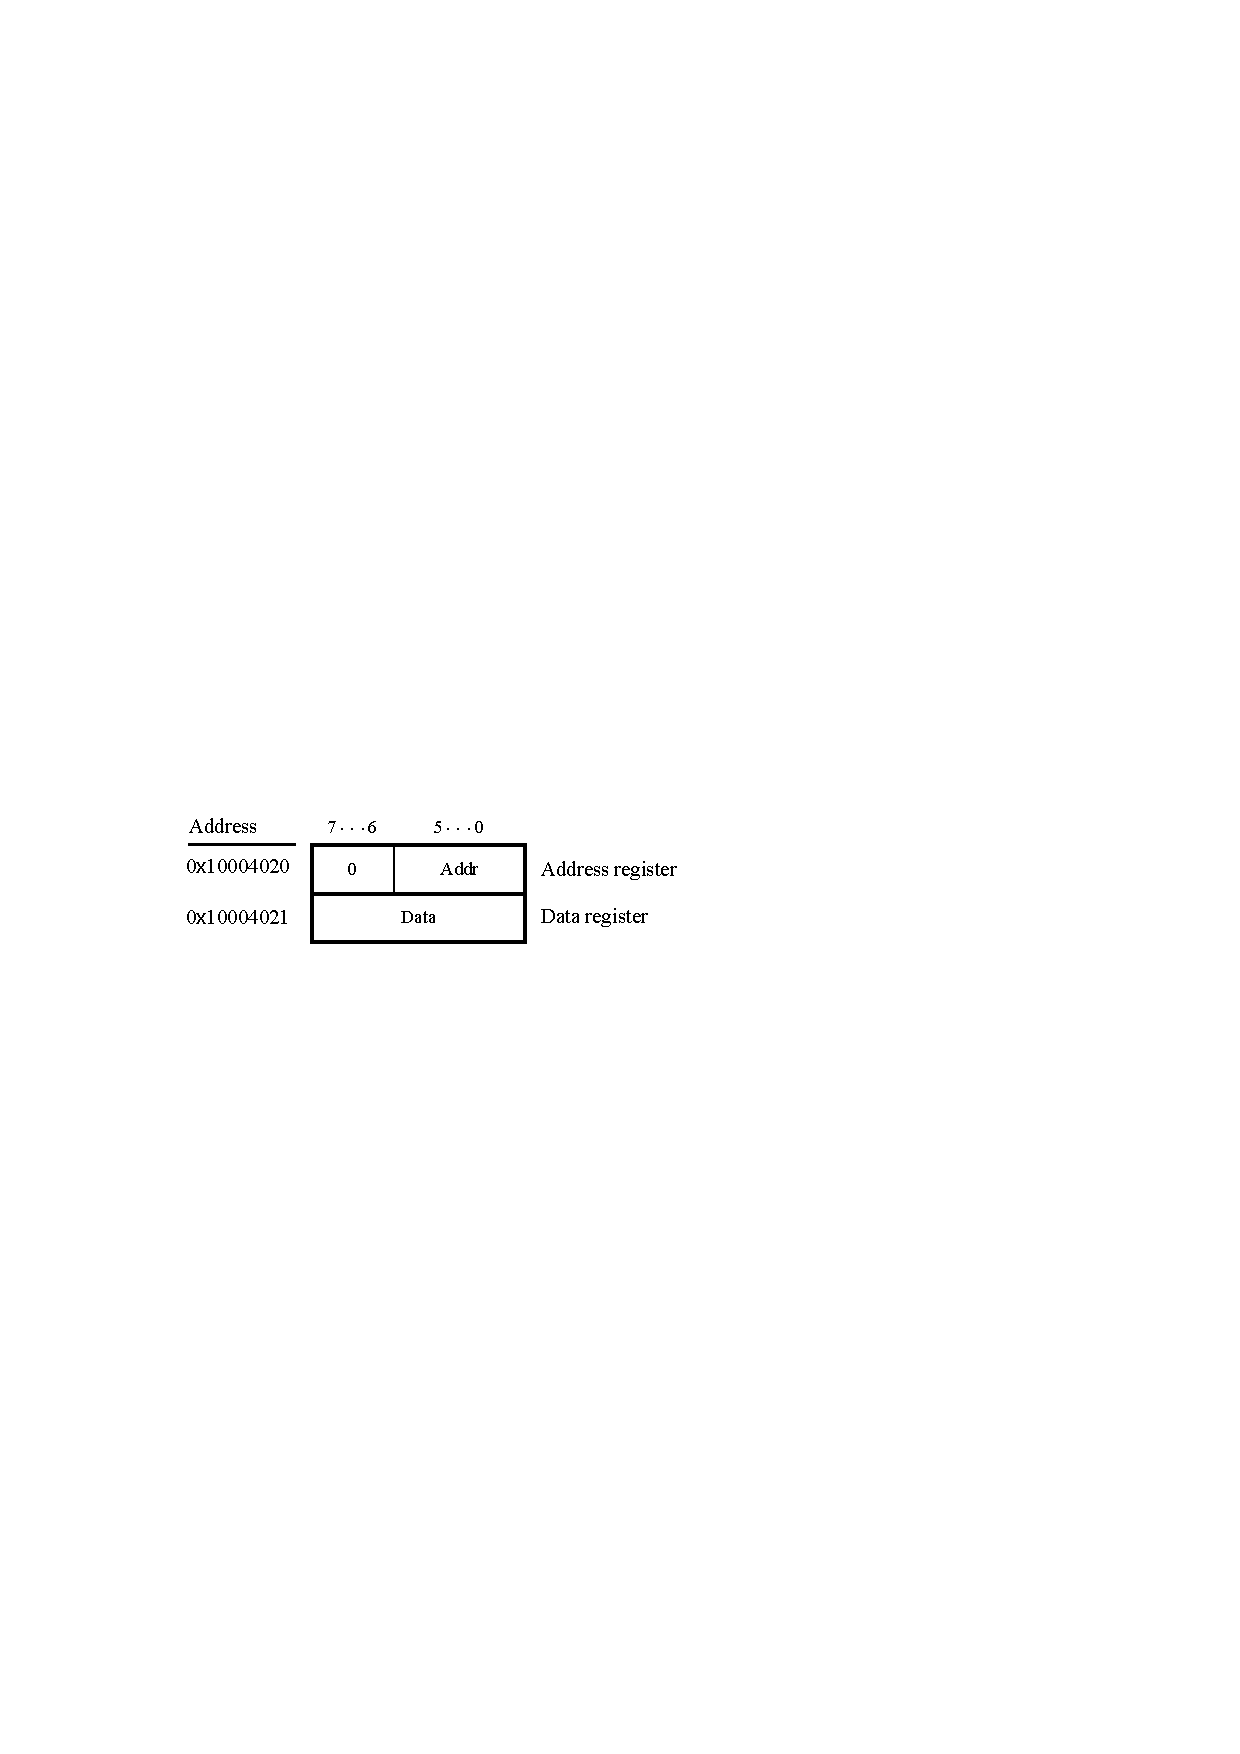
\includegraphics{\commonPath/../figs/FPGA_Accelerometer.pdf}
   \end{center}
   \caption{Accelerometer registers.}
	\label{fig:accel_port}
\end{figure}

The ADXL345 chip contains a series of 58 internal registers, {\sf 0x00} to {\sf 0x39}, which are
used to contol the device and store data. To access these registers, the address of the desired
register should be written to the {\it Address} register of the Accelerometer SPI Mode core.
Performing a read or write on the {\it Data} register will then read from or write to the 
requested address on the ADXL345. Commonly used registers of the accelerometer and their address
are listed in Table~\ref{tab:accel_regs}. For a full list of registers, consult the ADXL345 
datasheet.

\begin{table} [h]%
	\begin {center}
		\begin{tabular}{c|c|l}
			{\bf Address} &
			{\bf Register Name} &
			{\bf Description} \\
			\hline
			{\sf 0x32} & 
			{\it DATAX0} & 
			Low-order byte of {\it x}-axis acceleration. 
			\\
			{\sf 0x33} & 
			{\it DATAX1} & 
			High-order byte of {\it x}-axis acceleration.
			\\
			{\sf 0x34} & 
			{\it DATAY0} & 
			Low-order byte of {\it y}-axis acceleration. 
			\\
			{\sf 0x35} & 
			{\it DATAY1} & 
			High-order byte of {\it y}-axis acceleration.
			\\
			{\sf 0x36} & 
			{\it DATAZ0} & 
			Low-order byte of {\it z}-axis acceleration. 
			\\
			{\sf 0x37} & 
			{\it DATAZ1} & 
			High-order byte of {\it z}-axis acceleration.
			\\
		\end{tabular}
	\end{center}
\caption{Commonly used registers in the ADXL345 chip.}
\label{tab:accel_regs}
\end{table}